% Options for packages loaded elsewhere
\PassOptionsToPackage{unicode}{hyperref}
\PassOptionsToPackage{hyphens}{url}
\PassOptionsToPackage{dvipsnames,svgnames,x11names}{xcolor}
%
\documentclass[
  letterpaper,
  DIV=11,
  numbers=noendperiod]{scrreprt}

\usepackage{amsmath,amssymb}
\usepackage{iftex}
\ifPDFTeX
  \usepackage[T1]{fontenc}
  \usepackage[utf8]{inputenc}
  \usepackage{textcomp} % provide euro and other symbols
\else % if luatex or xetex
  \usepackage{unicode-math}
  \defaultfontfeatures{Scale=MatchLowercase}
  \defaultfontfeatures[\rmfamily]{Ligatures=TeX,Scale=1}
\fi
\usepackage{lmodern}
\ifPDFTeX\else  
    % xetex/luatex font selection
\fi
% Use upquote if available, for straight quotes in verbatim environments
\IfFileExists{upquote.sty}{\usepackage{upquote}}{}
\IfFileExists{microtype.sty}{% use microtype if available
  \usepackage[]{microtype}
  \UseMicrotypeSet[protrusion]{basicmath} % disable protrusion for tt fonts
}{}
\makeatletter
\@ifundefined{KOMAClassName}{% if non-KOMA class
  \IfFileExists{parskip.sty}{%
    \usepackage{parskip}
  }{% else
    \setlength{\parindent}{0pt}
    \setlength{\parskip}{6pt plus 2pt minus 1pt}}
}{% if KOMA class
  \KOMAoptions{parskip=half}}
\makeatother
\usepackage{xcolor}
\setlength{\emergencystretch}{3em} % prevent overfull lines
\setcounter{secnumdepth}{5}
% Make \paragraph and \subparagraph free-standing
\makeatletter
\ifx\paragraph\undefined\else
  \let\oldparagraph\paragraph
  \renewcommand{\paragraph}{
    \@ifstar
      \xxxParagraphStar
      \xxxParagraphNoStar
  }
  \newcommand{\xxxParagraphStar}[1]{\oldparagraph*{#1}\mbox{}}
  \newcommand{\xxxParagraphNoStar}[1]{\oldparagraph{#1}\mbox{}}
\fi
\ifx\subparagraph\undefined\else
  \let\oldsubparagraph\subparagraph
  \renewcommand{\subparagraph}{
    \@ifstar
      \xxxSubParagraphStar
      \xxxSubParagraphNoStar
  }
  \newcommand{\xxxSubParagraphStar}[1]{\oldsubparagraph*{#1}\mbox{}}
  \newcommand{\xxxSubParagraphNoStar}[1]{\oldsubparagraph{#1}\mbox{}}
\fi
\makeatother

\usepackage{color}
\usepackage{fancyvrb}
\newcommand{\VerbBar}{|}
\newcommand{\VERB}{\Verb[commandchars=\\\{\}]}
\DefineVerbatimEnvironment{Highlighting}{Verbatim}{commandchars=\\\{\}}
% Add ',fontsize=\small' for more characters per line
\usepackage{framed}
\definecolor{shadecolor}{RGB}{241,243,245}
\newenvironment{Shaded}{\begin{snugshade}}{\end{snugshade}}
\newcommand{\AlertTok}[1]{\textcolor[rgb]{0.68,0.00,0.00}{#1}}
\newcommand{\AnnotationTok}[1]{\textcolor[rgb]{0.37,0.37,0.37}{#1}}
\newcommand{\AttributeTok}[1]{\textcolor[rgb]{0.40,0.45,0.13}{#1}}
\newcommand{\BaseNTok}[1]{\textcolor[rgb]{0.68,0.00,0.00}{#1}}
\newcommand{\BuiltInTok}[1]{\textcolor[rgb]{0.00,0.23,0.31}{#1}}
\newcommand{\CharTok}[1]{\textcolor[rgb]{0.13,0.47,0.30}{#1}}
\newcommand{\CommentTok}[1]{\textcolor[rgb]{0.37,0.37,0.37}{#1}}
\newcommand{\CommentVarTok}[1]{\textcolor[rgb]{0.37,0.37,0.37}{\textit{#1}}}
\newcommand{\ConstantTok}[1]{\textcolor[rgb]{0.56,0.35,0.01}{#1}}
\newcommand{\ControlFlowTok}[1]{\textcolor[rgb]{0.00,0.23,0.31}{\textbf{#1}}}
\newcommand{\DataTypeTok}[1]{\textcolor[rgb]{0.68,0.00,0.00}{#1}}
\newcommand{\DecValTok}[1]{\textcolor[rgb]{0.68,0.00,0.00}{#1}}
\newcommand{\DocumentationTok}[1]{\textcolor[rgb]{0.37,0.37,0.37}{\textit{#1}}}
\newcommand{\ErrorTok}[1]{\textcolor[rgb]{0.68,0.00,0.00}{#1}}
\newcommand{\ExtensionTok}[1]{\textcolor[rgb]{0.00,0.23,0.31}{#1}}
\newcommand{\FloatTok}[1]{\textcolor[rgb]{0.68,0.00,0.00}{#1}}
\newcommand{\FunctionTok}[1]{\textcolor[rgb]{0.28,0.35,0.67}{#1}}
\newcommand{\ImportTok}[1]{\textcolor[rgb]{0.00,0.46,0.62}{#1}}
\newcommand{\InformationTok}[1]{\textcolor[rgb]{0.37,0.37,0.37}{#1}}
\newcommand{\KeywordTok}[1]{\textcolor[rgb]{0.00,0.23,0.31}{\textbf{#1}}}
\newcommand{\NormalTok}[1]{\textcolor[rgb]{0.00,0.23,0.31}{#1}}
\newcommand{\OperatorTok}[1]{\textcolor[rgb]{0.37,0.37,0.37}{#1}}
\newcommand{\OtherTok}[1]{\textcolor[rgb]{0.00,0.23,0.31}{#1}}
\newcommand{\PreprocessorTok}[1]{\textcolor[rgb]{0.68,0.00,0.00}{#1}}
\newcommand{\RegionMarkerTok}[1]{\textcolor[rgb]{0.00,0.23,0.31}{#1}}
\newcommand{\SpecialCharTok}[1]{\textcolor[rgb]{0.37,0.37,0.37}{#1}}
\newcommand{\SpecialStringTok}[1]{\textcolor[rgb]{0.13,0.47,0.30}{#1}}
\newcommand{\StringTok}[1]{\textcolor[rgb]{0.13,0.47,0.30}{#1}}
\newcommand{\VariableTok}[1]{\textcolor[rgb]{0.07,0.07,0.07}{#1}}
\newcommand{\VerbatimStringTok}[1]{\textcolor[rgb]{0.13,0.47,0.30}{#1}}
\newcommand{\WarningTok}[1]{\textcolor[rgb]{0.37,0.37,0.37}{\textit{#1}}}

\providecommand{\tightlist}{%
  \setlength{\itemsep}{0pt}\setlength{\parskip}{0pt}}\usepackage{longtable,booktabs,array}
\usepackage{calc} % for calculating minipage widths
% Correct order of tables after \paragraph or \subparagraph
\usepackage{etoolbox}
\makeatletter
\patchcmd\longtable{\par}{\if@noskipsec\mbox{}\fi\par}{}{}
\makeatother
% Allow footnotes in longtable head/foot
\IfFileExists{footnotehyper.sty}{\usepackage{footnotehyper}}{\usepackage{footnote}}
\makesavenoteenv{longtable}
\usepackage{graphicx}
\makeatletter
\def\maxwidth{\ifdim\Gin@nat@width>\linewidth\linewidth\else\Gin@nat@width\fi}
\def\maxheight{\ifdim\Gin@nat@height>\textheight\textheight\else\Gin@nat@height\fi}
\makeatother
% Scale images if necessary, so that they will not overflow the page
% margins by default, and it is still possible to overwrite the defaults
% using explicit options in \includegraphics[width, height, ...]{}
\setkeys{Gin}{width=\maxwidth,height=\maxheight,keepaspectratio}
% Set default figure placement to htbp
\makeatletter
\def\fps@figure{htbp}
\makeatother
% definitions for citeproc citations
\NewDocumentCommand\citeproctext{}{}
\NewDocumentCommand\citeproc{mm}{%
  \begingroup\def\citeproctext{#2}\cite{#1}\endgroup}
\makeatletter
 % allow citations to break across lines
 \let\@cite@ofmt\@firstofone
 % avoid brackets around text for \cite:
 \def\@biblabel#1{}
 \def\@cite#1#2{{#1\if@tempswa , #2\fi}}
\makeatother
\newlength{\cslhangindent}
\setlength{\cslhangindent}{1.5em}
\newlength{\csllabelwidth}
\setlength{\csllabelwidth}{3em}
\newenvironment{CSLReferences}[2] % #1 hanging-indent, #2 entry-spacing
 {\begin{list}{}{%
  \setlength{\itemindent}{0pt}
  \setlength{\leftmargin}{0pt}
  \setlength{\parsep}{0pt}
  % turn on hanging indent if param 1 is 1
  \ifodd #1
   \setlength{\leftmargin}{\cslhangindent}
   \setlength{\itemindent}{-1\cslhangindent}
  \fi
  % set entry spacing
  \setlength{\itemsep}{#2\baselineskip}}}
 {\end{list}}
\usepackage{calc}
\newcommand{\CSLBlock}[1]{\hfill\break\parbox[t]{\linewidth}{\strut\ignorespaces#1\strut}}
\newcommand{\CSLLeftMargin}[1]{\parbox[t]{\csllabelwidth}{\strut#1\strut}}
\newcommand{\CSLRightInline}[1]{\parbox[t]{\linewidth - \csllabelwidth}{\strut#1\strut}}
\newcommand{\CSLIndent}[1]{\hspace{\cslhangindent}#1}

\KOMAoption{captions}{tableheading}
\makeatletter
\@ifpackageloaded{tcolorbox}{}{\usepackage[skins,breakable]{tcolorbox}}
\@ifpackageloaded{fontawesome5}{}{\usepackage{fontawesome5}}
\definecolor{quarto-callout-color}{HTML}{909090}
\definecolor{quarto-callout-note-color}{HTML}{0758E5}
\definecolor{quarto-callout-important-color}{HTML}{CC1914}
\definecolor{quarto-callout-warning-color}{HTML}{EB9113}
\definecolor{quarto-callout-tip-color}{HTML}{00A047}
\definecolor{quarto-callout-caution-color}{HTML}{FC5300}
\definecolor{quarto-callout-color-frame}{HTML}{acacac}
\definecolor{quarto-callout-note-color-frame}{HTML}{4582ec}
\definecolor{quarto-callout-important-color-frame}{HTML}{d9534f}
\definecolor{quarto-callout-warning-color-frame}{HTML}{f0ad4e}
\definecolor{quarto-callout-tip-color-frame}{HTML}{02b875}
\definecolor{quarto-callout-caution-color-frame}{HTML}{fd7e14}
\makeatother
\makeatletter
\@ifpackageloaded{bookmark}{}{\usepackage{bookmark}}
\makeatother
\makeatletter
\@ifpackageloaded{caption}{}{\usepackage{caption}}
\AtBeginDocument{%
\ifdefined\contentsname
  \renewcommand*\contentsname{Table of contents}
\else
  \newcommand\contentsname{Table of contents}
\fi
\ifdefined\listfigurename
  \renewcommand*\listfigurename{List of Figures}
\else
  \newcommand\listfigurename{List of Figures}
\fi
\ifdefined\listtablename
  \renewcommand*\listtablename{List of Tables}
\else
  \newcommand\listtablename{List of Tables}
\fi
\ifdefined\figurename
  \renewcommand*\figurename{Figure}
\else
  \newcommand\figurename{Figure}
\fi
\ifdefined\tablename
  \renewcommand*\tablename{Table}
\else
  \newcommand\tablename{Table}
\fi
}
\@ifpackageloaded{float}{}{\usepackage{float}}
\floatstyle{ruled}
\@ifundefined{c@chapter}{\newfloat{codelisting}{h}{lop}}{\newfloat{codelisting}{h}{lop}[chapter]}
\floatname{codelisting}{Listing}
\newcommand*\listoflistings{\listof{codelisting}{List of Listings}}
\makeatother
\makeatletter
\makeatother
\makeatletter
\@ifpackageloaded{caption}{}{\usepackage{caption}}
\@ifpackageloaded{subcaption}{}{\usepackage{subcaption}}
\makeatother

\ifLuaTeX
  \usepackage{selnolig}  % disable illegal ligatures
\fi
\usepackage{bookmark}

\IfFileExists{xurl.sty}{\usepackage{xurl}}{} % add URL line breaks if available
\urlstyle{same} % disable monospaced font for URLs
\hypersetup{
  pdftitle={Multilevel Visualization},
  pdfauthor={Andrew Grogan-Kaylor},
  colorlinks=true,
  linkcolor={blue},
  filecolor={Maroon},
  citecolor={Blue},
  urlcolor={Blue},
  pdfcreator={LaTeX via pandoc}}


\title{Multilevel Visualization}
\author{Andrew Grogan-Kaylor}
\date{2024-10-15}

\begin{document}
\maketitle

\renewcommand*\contentsname{Table of contents}
{
\hypersetup{linkcolor=}
\setcounter{tocdepth}{2}
\tableofcontents
}
\listoffigures
\listoftables

\bookmarksetup{startatroot}

\chapter{Multilevel Visualization}\label{multilevel-visualization}

\begin{quote}
``Persist and verify\ldots{} The power that we abdicate to others out of
our insecurity - to others who insult us with their faux-intuition or
their authoritarian smugness - that comes back to hurt us so
deeply\ldots{} But the power we wrest from our own certitude - that
saves us.'' (Cash 2017)
\end{quote}

\section{Introduction}\label{introduction}

Below, I describe the use of \href{https://www.stata.com/}{Stata}
(StataCorp 2023), \href{https://www.r-project.org/}{R}\footnote{In R, I
  use the \texttt{ggplot2} (Wickham 2016) library.} (R Core Team 2023;
Wickham 2016), and \href{https://www.julialang.org/}{Julia} (Bezanson et
al. 2017) to visualize multilevel models.

\begin{tcolorbox}[enhanced jigsaw, colback=white, left=2mm, toprule=.15mm, arc=.35mm, colbacktitle=quarto-callout-tip-color!10!white, title=\textcolor{quarto-callout-tip-color}{\faLightbulb}\hspace{0.5em}{Comparison of Software}, bottomtitle=1mm, opacitybacktitle=0.6, bottomrule=.15mm, breakable, leftrule=.75mm, colframe=quarto-callout-tip-color-frame, toptitle=1mm, titlerule=0mm, coltitle=black, opacityback=0, rightrule=.15mm]

See my discussion of the advantages and disadvantages of different
software in the Appendix on estimation of multilevel models with
different software.

\end{tcolorbox}

\section{The Data}\label{sec-data}

\begin{tcolorbox}[enhanced jigsaw, colback=white, left=2mm, toprule=.15mm, arc=.35mm, colbacktitle=quarto-callout-note-color!10!white, title=\textcolor{quarto-callout-note-color}{\faInfo}\hspace{0.5em}{Dataset}, bottomtitle=1mm, opacitybacktitle=0.6, bottomrule=.15mm, breakable, leftrule=.75mm, colframe=quarto-callout-note-color-frame, toptitle=1mm, titlerule=0mm, coltitle=black, opacityback=0, rightrule=.15mm]

The examples use the \texttt{simulated\_multilevel\_data.dta} file. Here
is a
\href{https://github.com/agrogan1/multilevel-multilingual/raw/main/simulated_multilevel_data.dta}{direct
link} to download the data.

\end{tcolorbox}

\begin{longtable}[]{@{}
  >{\centering\arraybackslash}p{(\columnwidth - 12\tabcolsep) * \real{0.1266}}
  >{\centering\arraybackslash}p{(\columnwidth - 12\tabcolsep) * \real{0.0759}}
  >{\centering\arraybackslash}p{(\columnwidth - 12\tabcolsep) * \real{0.1139}}
  >{\centering\arraybackslash}p{(\columnwidth - 12\tabcolsep) * \real{0.0759}}
  >{\centering\arraybackslash}p{(\columnwidth - 12\tabcolsep) * \real{0.1392}}
  >{\centering\arraybackslash}p{(\columnwidth - 12\tabcolsep) * \real{0.1899}}
  >{\centering\arraybackslash}p{(\columnwidth - 12\tabcolsep) * \real{0.2785}}@{}}

\caption{\label{tbl-multilingual1}Sample of Simulated Multilevel Data}

\tabularnewline

\caption{Table continues below}\tabularnewline
\toprule\noalign{}
\begin{minipage}[b]{\linewidth}\centering
country
\end{minipage} & \begin{minipage}[b]{\linewidth}\centering
HDI
\end{minipage} & \begin{minipage}[b]{\linewidth}\centering
family
\end{minipage} & \begin{minipage}[b]{\linewidth}\centering
id
\end{minipage} & \begin{minipage}[b]{\linewidth}\centering
identity
\end{minipage} & \begin{minipage}[b]{\linewidth}\centering
intervention
\end{minipage} & \begin{minipage}[b]{\linewidth}\centering
physical\_punishment
\end{minipage} \\
\midrule\noalign{}
\endfirsthead
\toprule\noalign{}
\begin{minipage}[b]{\linewidth}\centering
country
\end{minipage} & \begin{minipage}[b]{\linewidth}\centering
HDI
\end{minipage} & \begin{minipage}[b]{\linewidth}\centering
family
\end{minipage} & \begin{minipage}[b]{\linewidth}\centering
id
\end{minipage} & \begin{minipage}[b]{\linewidth}\centering
identity
\end{minipage} & \begin{minipage}[b]{\linewidth}\centering
intervention
\end{minipage} & \begin{minipage}[b]{\linewidth}\centering
physical\_punishment
\end{minipage} \\
\midrule\noalign{}
\endhead
\bottomrule\noalign{}
\endlastfoot
1 & 69 & 1 & 1.1 & 1 & 0 & 3 \\
1 & 69 & 2 & 1.2 & 1 & 1 & 2 \\
1 & 69 & 3 & 1.3 & 0 & 1 & 3 \\
1 & 69 & 4 & 1.4 & 1 & 0 & 0 \\
1 & 69 & 5 & 1.5 & 1 & 0 & 4 \\
1 & 69 & 6 & 1.6 & 0 & 1 & 5 \\

\end{longtable}

\begin{longtable}[]{@{}
  >{\centering\arraybackslash}p{(\columnwidth - 2\tabcolsep) * \real{0.1250}}
  >{\centering\arraybackslash}p{(\columnwidth - 2\tabcolsep) * \real{0.1389}}@{}}

\caption{\label{tbl-multilingual1}Sample of Simulated Multilevel Data}

\tabularnewline

\toprule\noalign{}
\begin{minipage}[b]{\linewidth}\centering
warmth
\end{minipage} & \begin{minipage}[b]{\linewidth}\centering
outcome
\end{minipage} \\
\midrule\noalign{}
\endhead
\bottomrule\noalign{}
\endlastfoot
3 & 57.47 \\
1 & 50.1 \\
2 & 52.92 \\
5 & 60.17 \\
4 & 55.05 \\
3 & 49.81 \\

\end{longtable}

\bookmarksetup{startatroot}

\chapter{Graphs}\label{graphs}

\begin{tcolorbox}[enhanced jigsaw, colback=white, left=2mm, toprule=.15mm, arc=.35mm, colbacktitle=quarto-callout-caution-color!10!white, title=\textcolor{quarto-callout-caution-color}{\faFire}\hspace{0.5em}{Order of Variables}, bottomtitle=1mm, opacitybacktitle=0.6, bottomrule=.15mm, breakable, leftrule=.75mm, colframe=quarto-callout-caution-color-frame, toptitle=1mm, titlerule=0mm, coltitle=black, opacityback=0, rightrule=.15mm]

Across software platforms, pay attention to the order of variables. I
generally use \texttt{x} for an \emph{independent} variable along the
horizontal axis and \texttt{y} for a \emph{dependent} variable along the
vertical axis. Different software asks for the variables to be listed in
different order, or different ways, so it is worth paying close
attention to the syntax.

\end{tcolorbox}

\section{Scatterplots}\label{scatterplots}

A scatterplot is one of the most basic of all data visualizations. At
the same time, a scatterplot can be tremendously informative because it
provides: the location of every data point (data points may be
overprinted); a sense of the distribution of both the \emph{x} and
\emph{y} variables; and a sense of the overall trend in the relationship
between the two variables, if there is one.

\subsection{Stata}

\subsubsection{Get The Data}\label{get-the-data}

\begin{Shaded}
\begin{Highlighting}[]

\KeywordTok{use}\NormalTok{ simulated\_multilevel\_data.dta}
\end{Highlighting}
\end{Shaded}

\subsubsection{Scatterplot}\label{scatterplot}

\begin{Shaded}
\begin{Highlighting}[]
\KeywordTok{twoway} \KeywordTok{scatter}\NormalTok{ outcome warmth, }\CommentTok{///}
  \BaseNTok{xtitle}\NormalTok{(}\StringTok{"warmth"}\NormalTok{) }\BaseNTok{ytitle}\NormalTok{(}\StringTok{"outcome"}\NormalTok{) }\CommentTok{///}
  \BaseNTok{title}\NormalTok{(}\StringTok{"Outcome by Parental Warmth"}\NormalTok{) }

\KeywordTok{quietly} \KeywordTok{graph} \KeywordTok{export} \KeywordTok{scatter}\NormalTok{.png, }\KeywordTok{replace}
\end{Highlighting}
\end{Shaded}

\begin{figure}

\centering{

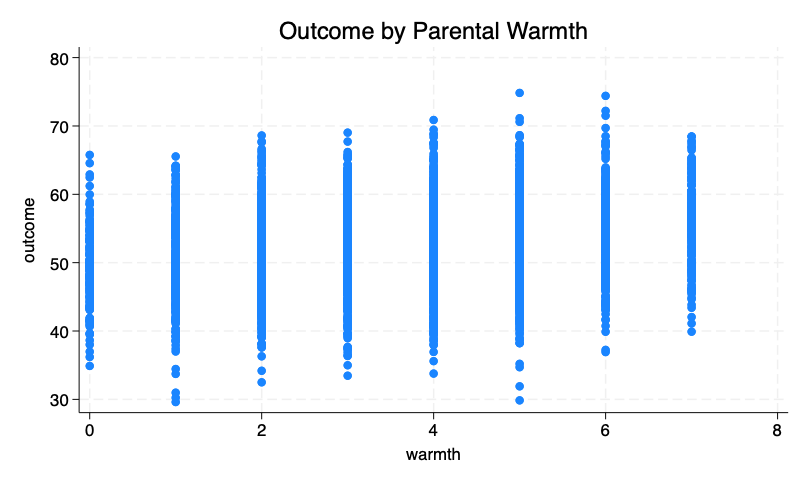
\includegraphics{scatter.png}

}

\caption{\label{fig-Stata}Outcome by Parental Warmth (Stata)}

\end{figure}%

\subsection{R}

\subsubsection{Get The Data}\label{get-the-data-1}

\begin{Shaded}
\begin{Highlighting}[]
\FunctionTok{library}\NormalTok{(haven)}

\NormalTok{df }\OtherTok{\textless{}{-}} \FunctionTok{read\_dta}\NormalTok{(}\StringTok{"simulated\_multilevel\_data.dta"}\NormalTok{)}
\end{Highlighting}
\end{Shaded}

\subsubsection{Scatterplot}\label{scatterplot-1}

\begin{Shaded}
\begin{Highlighting}[]
\FunctionTok{library}\NormalTok{(ggplot2)}

\FunctionTok{ggplot}\NormalTok{(df,}
       \FunctionTok{aes}\NormalTok{(}\AttributeTok{x =}\NormalTok{ warmth,}
           \AttributeTok{y =}\NormalTok{ outcome)) }\SpecialCharTok{+}
  \FunctionTok{geom\_point}\NormalTok{() }\SpecialCharTok{+}
  \FunctionTok{labs}\NormalTok{(}\AttributeTok{title =} \StringTok{"Outcome by Parental Warmth"}\NormalTok{)}
\end{Highlighting}
\end{Shaded}

\begin{figure}[H]

\centering{

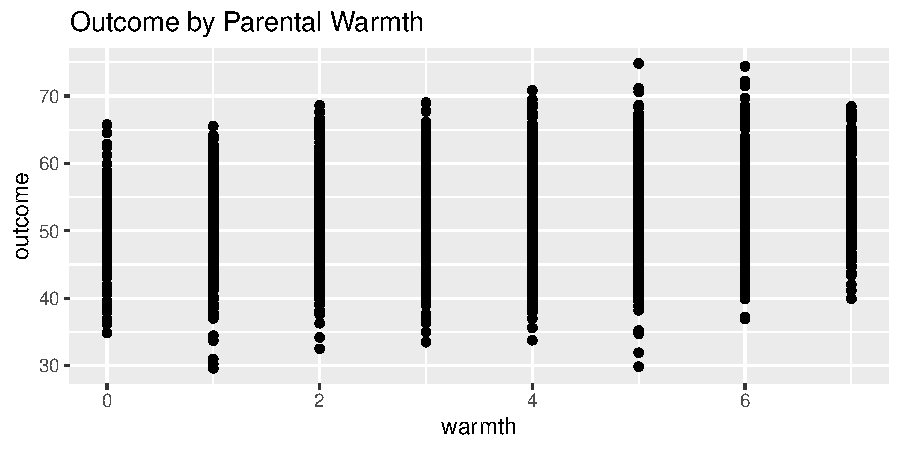
\includegraphics{graphs_files/figure-pdf/fig-R-1.pdf}

}

\caption{\label{fig-R}Outcome by Parental Warmth (R)}

\end{figure}%

\subsection{Julia}

\subsubsection{Get The Data}\label{get-the-data-2}

\begin{Shaded}
\begin{Highlighting}[]
\ImportTok{using} \BuiltInTok{Tables}\NormalTok{, }\BuiltInTok{MixedModels}\NormalTok{, }\BuiltInTok{StatFiles}\NormalTok{, }\BuiltInTok{DataFrames}\NormalTok{, }\BuiltInTok{CategoricalArrays}\NormalTok{, }\BuiltInTok{DataFramesMeta}

\NormalTok{df }\OperatorTok{=} \FunctionTok{DataFrame}\NormalTok{(}\FunctionTok{load}\NormalTok{(}\StringTok{"simulated\_multilevel\_data.dta"}\NormalTok{))}
\end{Highlighting}
\end{Shaded}

\subsubsection{Scatterplot}\label{scatterplot-2}

\begin{Shaded}
\begin{Highlighting}[]
\ImportTok{using} \BuiltInTok{StatsPlots}

\PreprocessorTok{@df}\NormalTok{ df }\FunctionTok{scatter}\NormalTok{(}\OperatorTok{:}\NormalTok{warmth, }\OperatorTok{:}\NormalTok{outcome, }
\NormalTok{               title }\OperatorTok{=} \StringTok{"Outcome by Parental Warmth"}\NormalTok{,}
\NormalTok{               ylabel }\OperatorTok{=} \StringTok{"outcome"}\NormalTok{,}
\NormalTok{               xlabel }\OperatorTok{=} \StringTok{"parental warmth"}\NormalTok{)}
\end{Highlighting}
\end{Shaded}

\begin{figure}[H]

\centering{

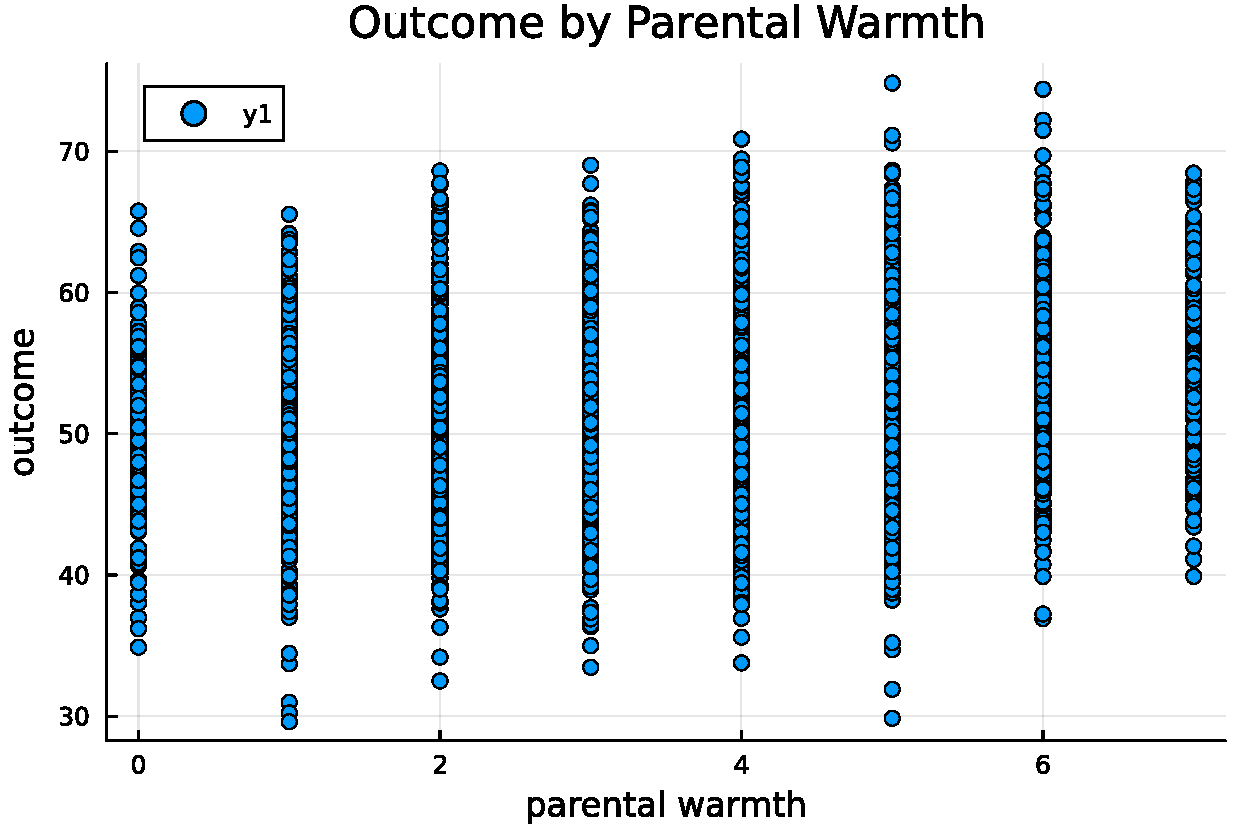
\includegraphics{graphs_files/figure-pdf/fig-Julia-J1.pdf}

}

\caption{\label{fig-Julia}Outcome by Parental Warmth (Julia)}

\end{figure}%

\section{Line Graph (Linear Trend)}\label{line-graph-linear-trend}

A line graph of the data focuses in on the linear trend in the data.

\subsection{Stata}

\subsubsection{Get The Data}\label{get-the-data-3}

\begin{Shaded}
\begin{Highlighting}[]

\KeywordTok{use}\NormalTok{ simulated\_multilevel\_data.dta}
\end{Highlighting}
\end{Shaded}

\subsubsection{Line Graph}\label{line-graph}

\begin{Shaded}
\begin{Highlighting}[]
\KeywordTok{twoway} \KeywordTok{lfit}\NormalTok{ outcome warmth, }\CommentTok{///}
  \BaseNTok{xtitle}\NormalTok{(}\StringTok{"warmth"}\NormalTok{) }\BaseNTok{ytitle}\NormalTok{(}\StringTok{"outcome"}\NormalTok{) }\CommentTok{///}
  \BaseNTok{title}\NormalTok{(}\StringTok{"Outcome by Parental Warmth"}\NormalTok{) }

\KeywordTok{quietly} \KeywordTok{graph} \KeywordTok{export} \KeywordTok{lfit}\NormalTok{.png, }\KeywordTok{replace}
\end{Highlighting}
\end{Shaded}

\begin{figure}

\centering{

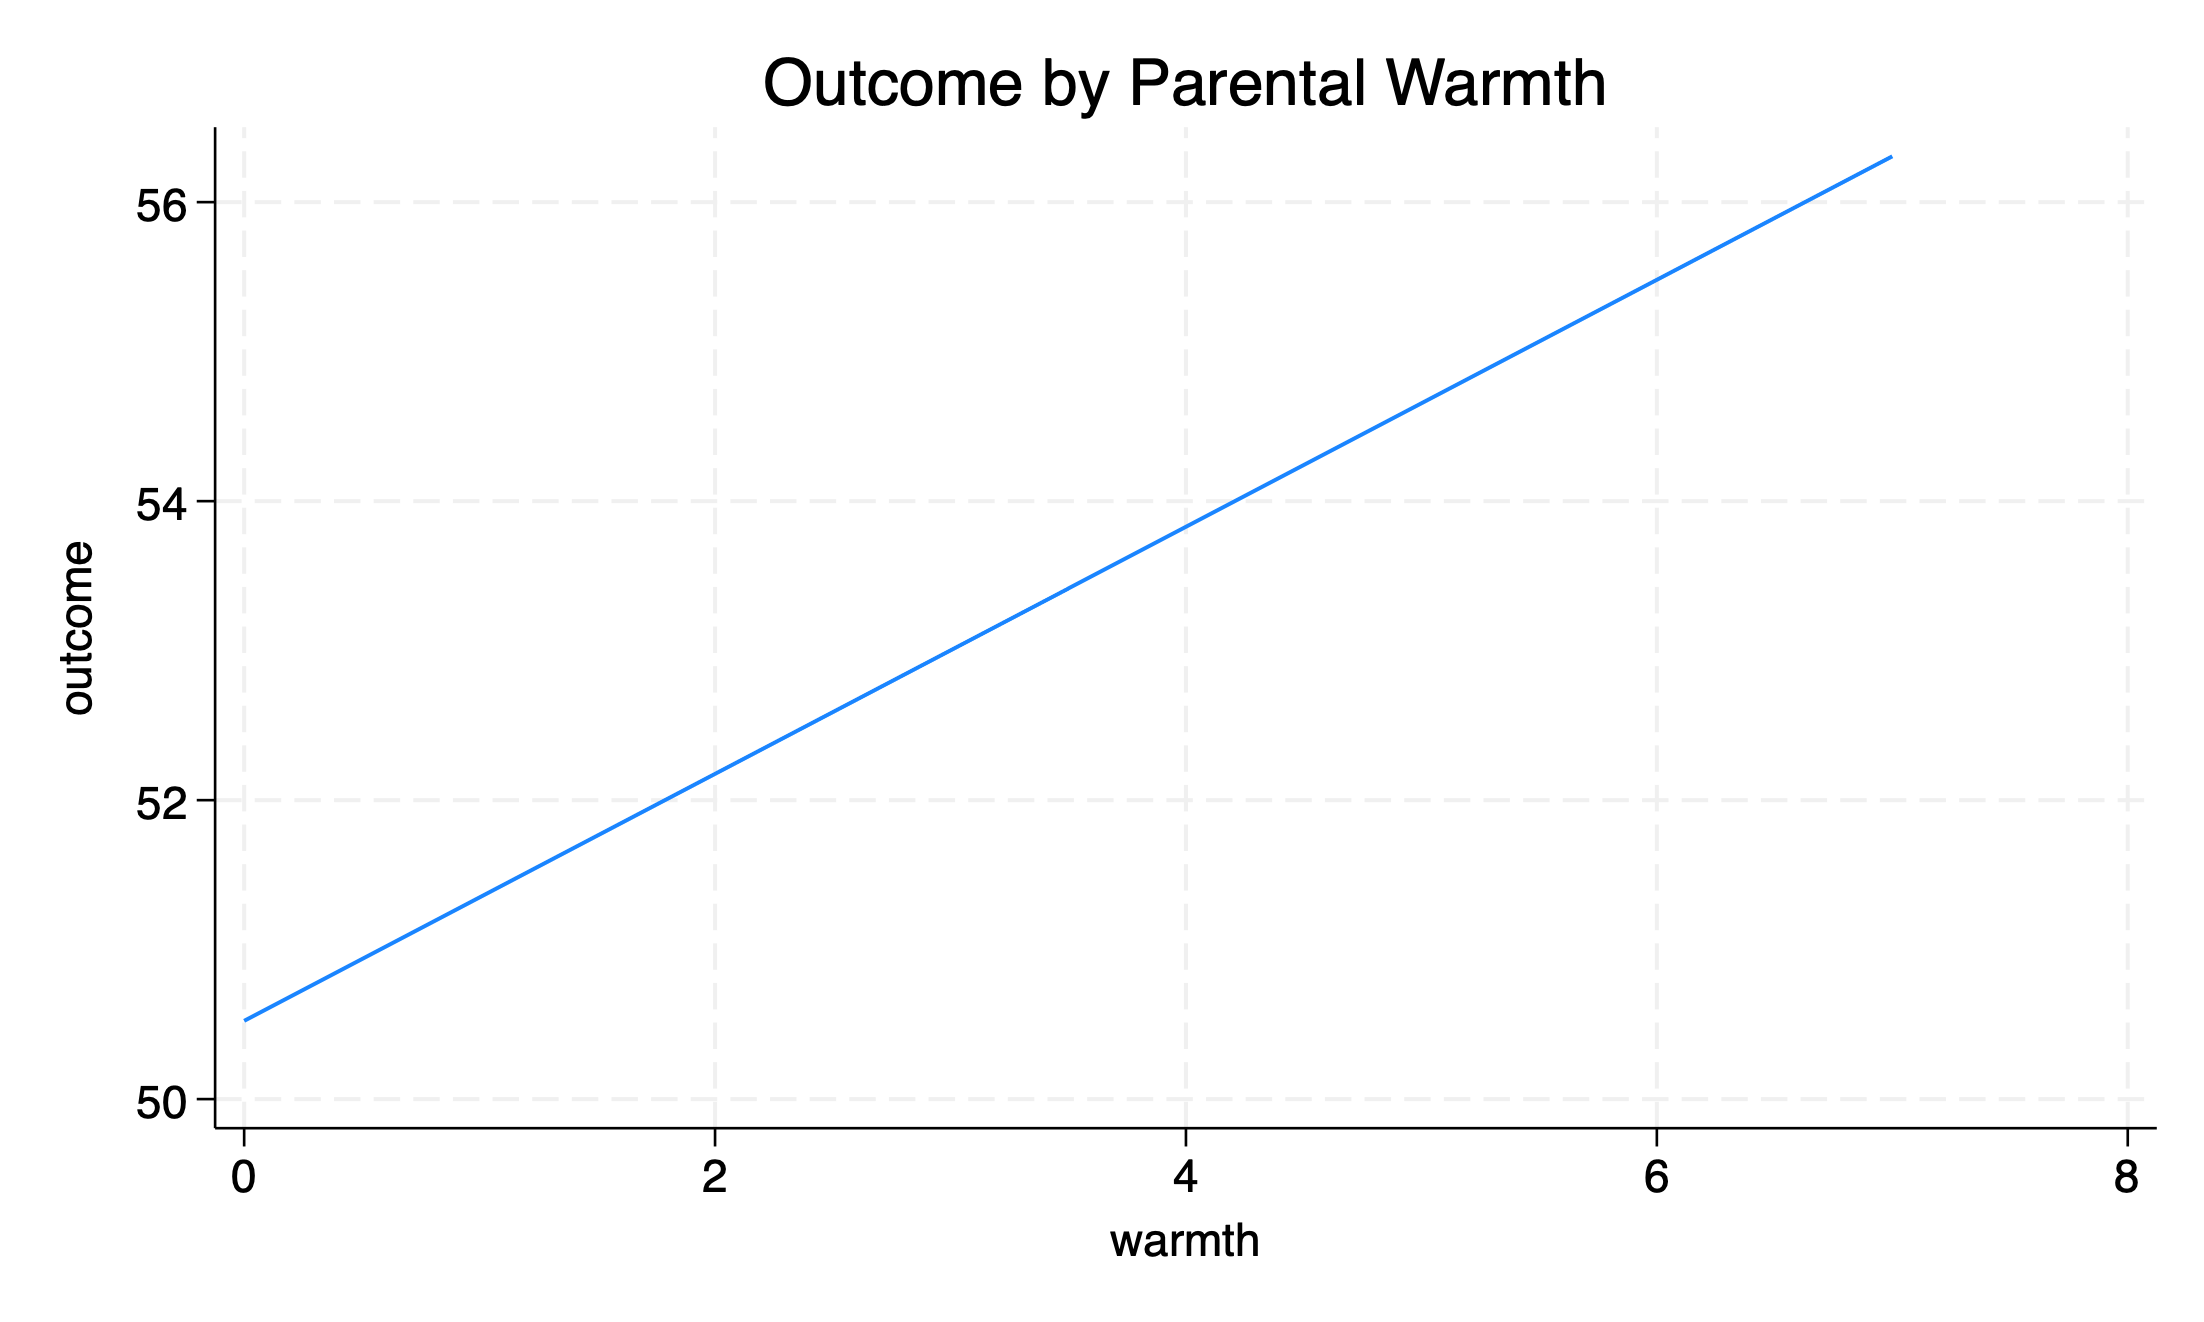
\includegraphics{lfit.png}

}

\caption{\label{fig-Statalfit}Outcome by Parental Warmth (Stata)}

\end{figure}%

\subsection{R}

\subsubsection{Get The Data}\label{get-the-data-4}

\begin{Shaded}
\begin{Highlighting}[]
\FunctionTok{library}\NormalTok{(haven)}

\NormalTok{df }\OtherTok{\textless{}{-}} \FunctionTok{read\_dta}\NormalTok{(}\StringTok{"simulated\_multilevel\_data.dta"}\NormalTok{)}
\end{Highlighting}
\end{Shaded}

\subsubsection{Line Graph}\label{line-graph-1}

\begin{Shaded}
\begin{Highlighting}[]
\FunctionTok{library}\NormalTok{(ggplot2)}

\FunctionTok{ggplot}\NormalTok{(df,}
       \FunctionTok{aes}\NormalTok{(}\AttributeTok{y =}\NormalTok{ outcome,}
           \AttributeTok{x =}\NormalTok{ warmth)) }\SpecialCharTok{+}
  \FunctionTok{geom\_smooth}\NormalTok{(}\AttributeTok{method =} \StringTok{"lm"}\NormalTok{) }\SpecialCharTok{+}
\FunctionTok{labs}\NormalTok{(}\AttributeTok{title =} \StringTok{"Outcome by Parental Warmth"}\NormalTok{)}
\end{Highlighting}
\end{Shaded}

\begin{figure}[H]

\centering{

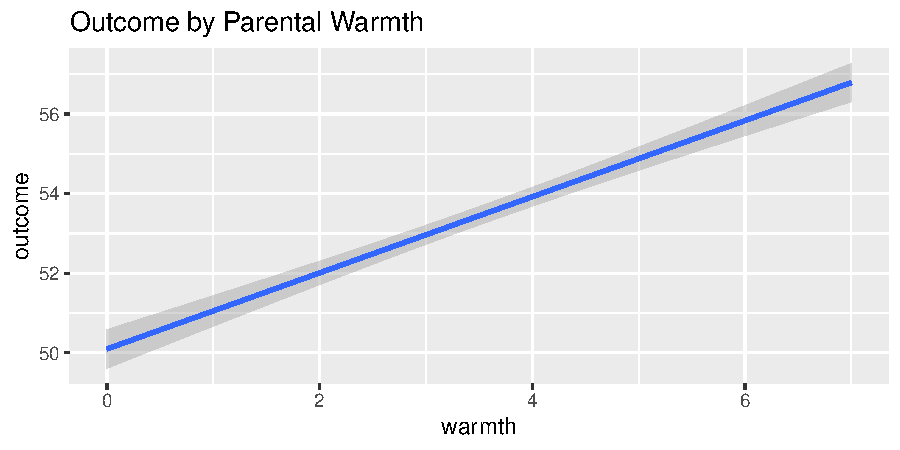
\includegraphics{graphs_files/figure-pdf/fig-Rlfit-1.pdf}

}

\caption{\label{fig-Rlfit}Outcome by Parental Warmth (R)}

\end{figure}%

\subsection{Julia}

\subsubsection{Get The Data}\label{get-the-data-5}

\begin{Shaded}
\begin{Highlighting}[]
\ImportTok{using} \BuiltInTok{Tables}\NormalTok{, }\BuiltInTok{MixedModels}\NormalTok{, }\BuiltInTok{StatFiles}\NormalTok{, }\BuiltInTok{DataFrames}\NormalTok{, }\BuiltInTok{CategoricalArrays}\NormalTok{, }\BuiltInTok{DataFramesMeta}

\NormalTok{df }\OperatorTok{=} \FunctionTok{DataFrame}\NormalTok{(}\FunctionTok{load}\NormalTok{(}\StringTok{"simulated\_multilevel\_data.dta"}\NormalTok{))}
\end{Highlighting}
\end{Shaded}

\subsubsection{Line Graph}\label{line-graph-2}

To make our plot with a smoother in Julia, we set the
\texttt{markercolor} and \texttt{markerstrokecolor} to be \emph{white},
and the \texttt{smooth} option to \texttt{:true}.

\begin{Shaded}
\begin{Highlighting}[]
\ImportTok{using} \BuiltInTok{StatsPlots}

\PreprocessorTok{@df}\NormalTok{ df }\FunctionTok{scatter}\NormalTok{(}\OperatorTok{:}\NormalTok{warmth, }\OperatorTok{:}\NormalTok{outcome, }
\NormalTok{               title }\OperatorTok{=} \StringTok{"Outcome by Parental Warmth"}\NormalTok{,}
\NormalTok{               ylabel }\OperatorTok{=} \StringTok{"outcome"}\NormalTok{,}
\NormalTok{               xlabel }\OperatorTok{=} \StringTok{"warmth"}\NormalTok{,}
\NormalTok{               markercolor }\OperatorTok{=} \StringTok{"white"}\NormalTok{,}
\NormalTok{               markerstrokecolor }\OperatorTok{=} \StringTok{"white"}\NormalTok{,}
\NormalTok{               smooth}\OperatorTok{=:}\ConstantTok{true}\NormalTok{)}
\end{Highlighting}
\end{Shaded}

\begin{figure}[H]

\centering{

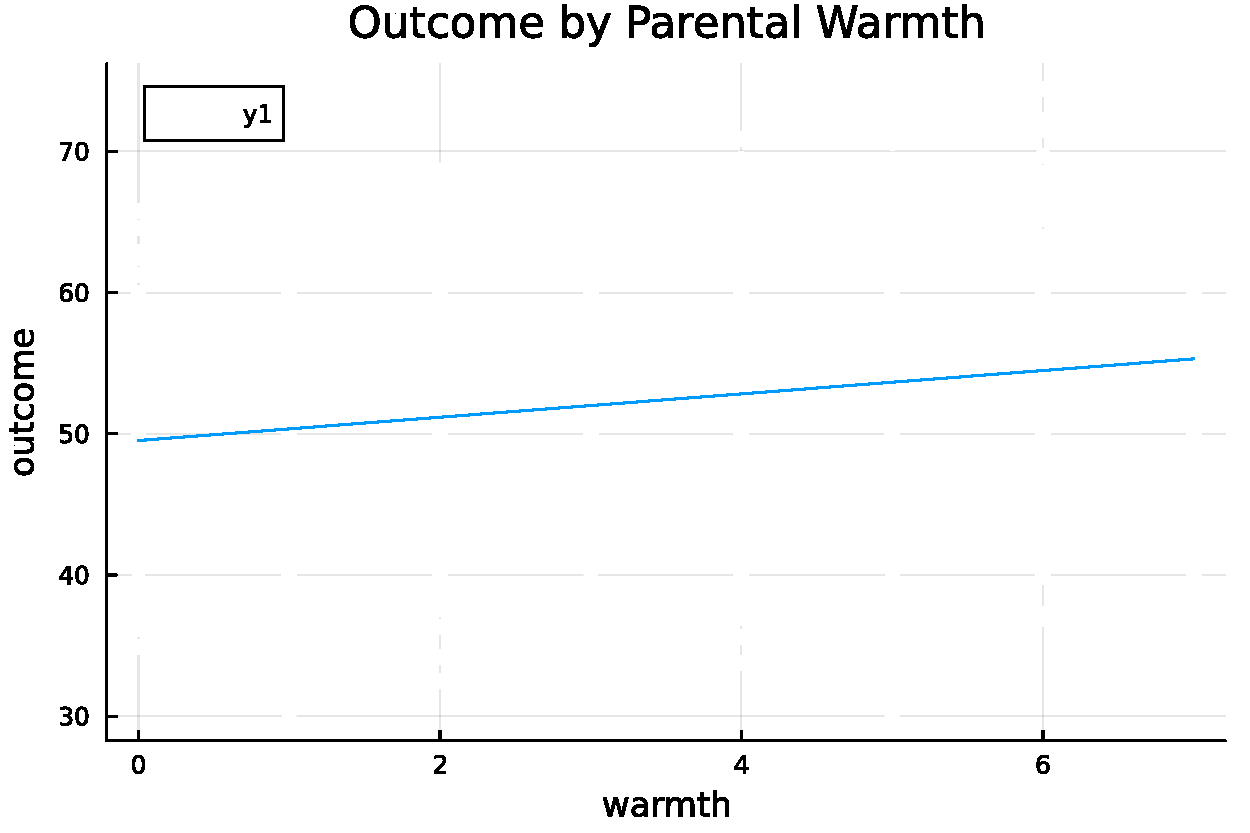
\includegraphics{graphs_files/figure-pdf/fig-Julialfit-J1.pdf}

}

\caption{\label{fig-Julialfit}Outcome by Parental Warmth (Julia)}

\end{figure}%

\section{Spaghetti Plots}\label{spaghetti-plots}

A \emph{spaghetti plot} might be considered the most \emph{multilevel}
of the visualizations here considered. A spaghetti plot shows the group
specific slopes and intercepts for all of the groups in the data.

\subsection{Stata}

In Stata, spaghetti plots are most easily generated using the user
written \texttt{spagplot} command. Type \texttt{findit\ spagplot} to
install this command.

\subsubsection{Get The Data}\label{get-the-data-6}

\begin{Shaded}
\begin{Highlighting}[]

\KeywordTok{use}\NormalTok{ simulated\_multilevel\_data.dta}
\end{Highlighting}
\end{Shaded}

\subsubsection{Spaghetti Plot}\label{spaghetti-plot}

\begin{tcolorbox}[enhanced jigsaw, colback=white, left=2mm, toprule=.15mm, arc=.35mm, colbacktitle=quarto-callout-tip-color!10!white, title=\textcolor{quarto-callout-tip-color}{\faLightbulb}\hspace{0.5em}{Installing \texttt{spagplot}}, bottomtitle=1mm, opacitybacktitle=0.6, bottomrule=.15mm, breakable, leftrule=.75mm, colframe=quarto-callout-tip-color-frame, toptitle=1mm, titlerule=0mm, coltitle=black, opacityback=0, rightrule=.15mm]

\texttt{spagplot} is a user written command. Type
\texttt{findit\ spagplot} to install.

\end{tcolorbox}

\begin{Shaded}
\begin{Highlighting}[]
\NormalTok{spagplot outcome warmth, }\CommentTok{///}
\NormalTok{  id(country) }\CommentTok{///}
  \BaseNTok{xtitle}\NormalTok{(}\StringTok{"parental warmth"}\NormalTok{) }\BaseNTok{ytitle}\NormalTok{(}\StringTok{"outcome"}\NormalTok{) }\CommentTok{///}
  \BaseNTok{title}\NormalTok{(}\StringTok{"Outcome by Parental Warmth"}\NormalTok{) }

\KeywordTok{quietly} \KeywordTok{graph} \KeywordTok{export}\NormalTok{ spagplot.png, }\KeywordTok{replace}
\end{Highlighting}
\end{Shaded}

\begin{figure}

\centering{

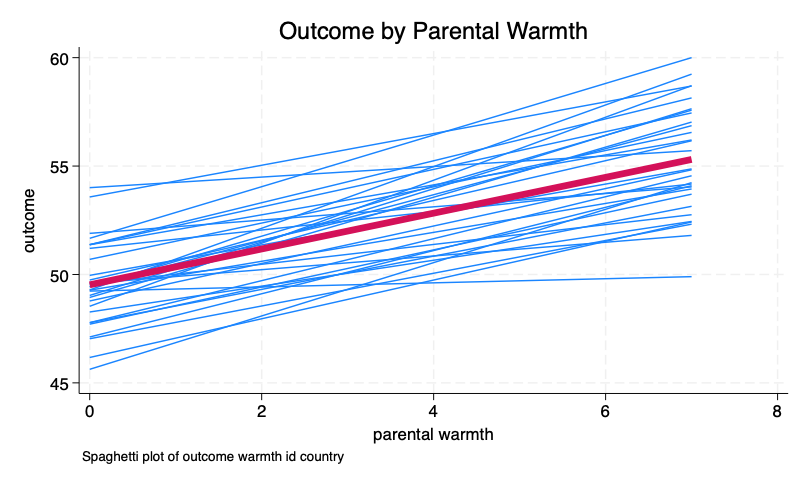
\includegraphics{spagplot.png}

}

\caption{\label{fig-Stataspagplot}Outcome by Parental Warmth (Stata)}

\end{figure}%

\subsection{R}

\subsubsection{Get The Data}\label{get-the-data-7}

\begin{Shaded}
\begin{Highlighting}[]
\FunctionTok{library}\NormalTok{(haven)}

\NormalTok{df }\OtherTok{\textless{}{-}} \FunctionTok{read\_dta}\NormalTok{(}\StringTok{"simulated\_multilevel\_data.dta"}\NormalTok{)}
\end{Highlighting}
\end{Shaded}

\subsubsection{Spaghetti Plot}\label{spaghetti-plot-1}

\begin{Shaded}
\begin{Highlighting}[]
\FunctionTok{library}\NormalTok{(ggplot2)}

\NormalTok{df}\SpecialCharTok{$}\NormalTok{country }\OtherTok{\textless{}{-}} \FunctionTok{factor}\NormalTok{(df}\SpecialCharTok{$}\NormalTok{country)}

\FunctionTok{ggplot}\NormalTok{(df,}
       \FunctionTok{aes}\NormalTok{(}\AttributeTok{y =}\NormalTok{ outcome,}
           \AttributeTok{x =}\NormalTok{ warmth)) }\SpecialCharTok{+}
  \FunctionTok{geom\_smooth}\NormalTok{(}\FunctionTok{aes}\NormalTok{(}\AttributeTok{color =}\NormalTok{ country,}
                  \AttributeTok{group =}\NormalTok{ country), }
              \AttributeTok{method =} \StringTok{"lm"}\NormalTok{,}
              \AttributeTok{se =} \ConstantTok{FALSE}\NormalTok{) }\SpecialCharTok{+}
    \FunctionTok{geom\_smooth}\NormalTok{(}\AttributeTok{method =} \StringTok{"lm"}\NormalTok{, }\AttributeTok{linewidth =} \DecValTok{3}\NormalTok{) }\SpecialCharTok{+}
\FunctionTok{labs}\NormalTok{(}\AttributeTok{title =} \StringTok{"Outcome by Parental Warmth"}\NormalTok{)}
\end{Highlighting}
\end{Shaded}

\begin{figure}[H]

\centering{

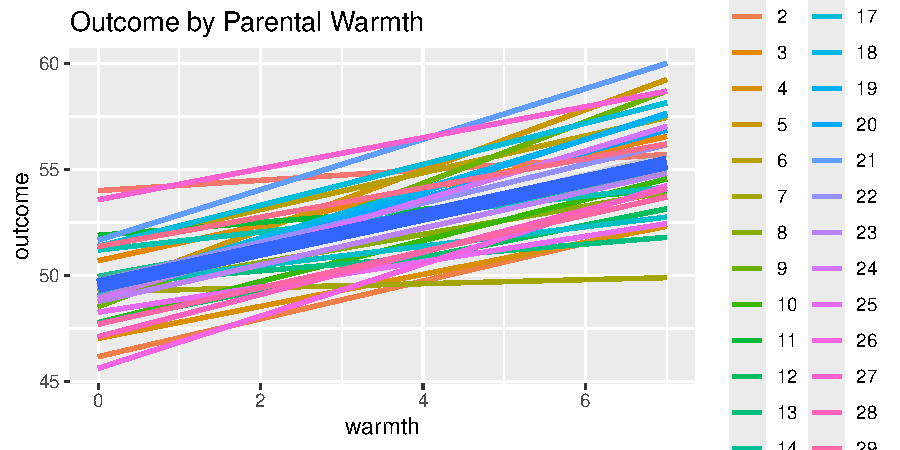
\includegraphics{graphs_files/figure-pdf/fig-Rspagplot-1.pdf}

}

\caption{\label{fig-Rspagplot}Outcome by Parental Warmth (R)}

\end{figure}%

\subsection{Julia}

\subsubsection{Get The Data}\label{get-the-data-8}

\begin{Shaded}
\begin{Highlighting}[]
\ImportTok{using} \BuiltInTok{Tables}\NormalTok{, }\BuiltInTok{MixedModels}\NormalTok{, }\BuiltInTok{StatFiles}\NormalTok{, }\BuiltInTok{DataFrames}\NormalTok{, }\BuiltInTok{CategoricalArrays}\NormalTok{, }\BuiltInTok{DataFramesMeta}

\NormalTok{df }\OperatorTok{=} \FunctionTok{DataFrame}\NormalTok{(}\FunctionTok{load}\NormalTok{(}\StringTok{"simulated\_multilevel\_data.dta"}\NormalTok{))}
\end{Highlighting}
\end{Shaded}

\subsubsection{Spaghetti Plot}\label{spaghetti-plot-2}

\begin{Shaded}
\begin{Highlighting}[]
\ImportTok{using} \BuiltInTok{StatsPlots}

\PreprocessorTok{@df}\NormalTok{ df }\FunctionTok{scatter}\NormalTok{(}\OperatorTok{:}\NormalTok{warmth, }\OperatorTok{:}\NormalTok{outcome, }
\NormalTok{               title }\OperatorTok{=} \StringTok{"Outcome by Parental Warmth"}\NormalTok{,}
\NormalTok{               ylabel }\OperatorTok{=} \StringTok{"outcome"}\NormalTok{,}
\NormalTok{               xlabel }\OperatorTok{=} \StringTok{"warmth"}\NormalTok{,}
\NormalTok{               markercolor }\OperatorTok{=} \StringTok{"white"}\NormalTok{,}
\NormalTok{               markerstrokecolor }\OperatorTok{=} \StringTok{"white"}\NormalTok{,}
\NormalTok{               group }\OperatorTok{=} \OperatorTok{:}\NormalTok{country,}
\NormalTok{               legend }\OperatorTok{=} \ConstantTok{false}\NormalTok{,}
\NormalTok{               smooth}\OperatorTok{=:}\ConstantTok{true}\NormalTok{)}
\end{Highlighting}
\end{Shaded}

\begin{figure}[H]

\centering{

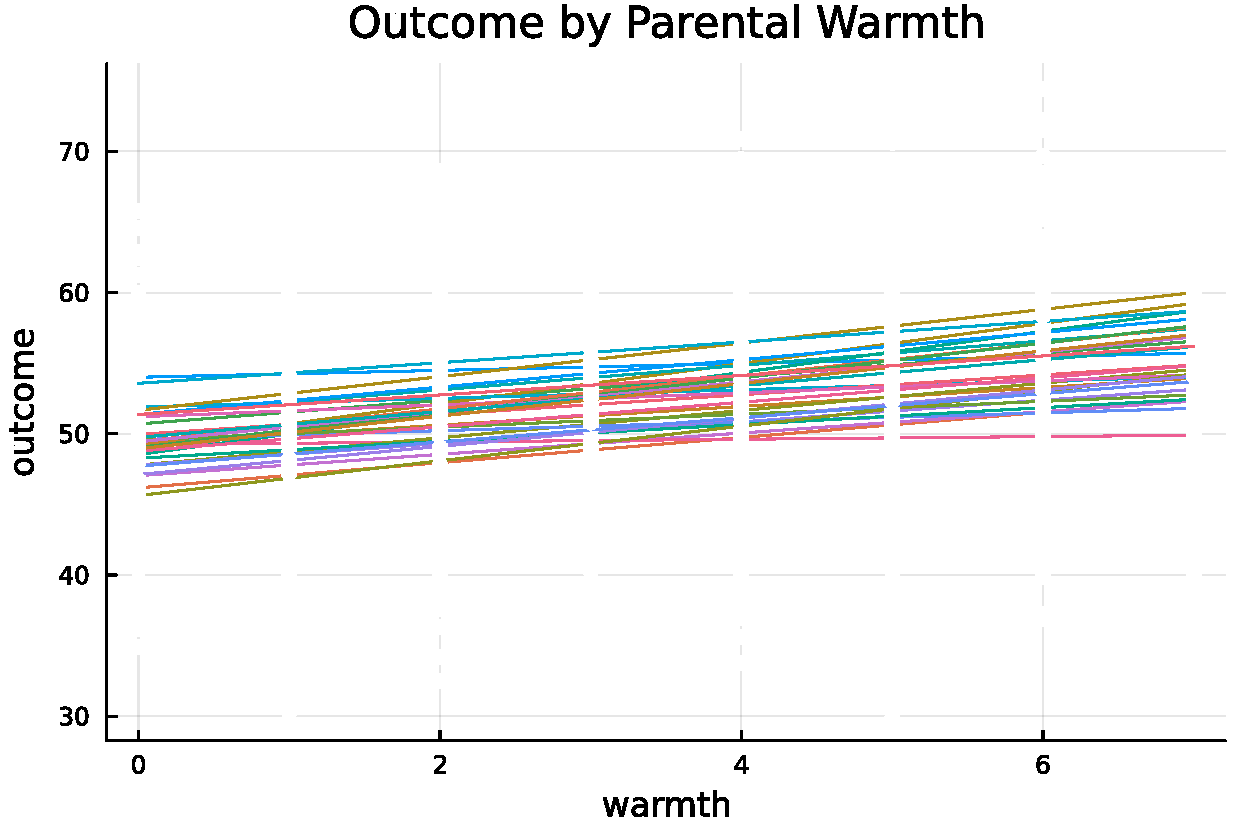
\includegraphics{graphs_files/figure-pdf/fig-Juliaspagplot-J1.pdf}

}

\caption{\label{fig-Juliaspagplot}Outcome by Parental Warmth (Julia)}

\end{figure}%

\bookmarksetup{startatroot}

\chapter*{References}\label{references}
\addcontentsline{toc}{chapter}{References}

\markboth{References}{References}

\phantomsection\label{refs}
\begin{CSLReferences}{1}{0}
\bibitem[\citeproctext]{ref-JuliaArticle}
Bezanson, Jeff, Alan Edelman, Stefan Karpinski, and Viral B. Shah. 2017.
{``Julia: A Fresh Approach to Numerical Computing.''} \emph{SIAM Review}
59 (1): 65--98. \url{https://doi.org/10.1137/141000671}.

\bibitem[\citeproctext]{ref-Cash2017}
Cash, Roseanne. 2017. {``Roseanne Cash Reads 'Power' by Adrienne
Rich.''} In \emph{The Universe in Verse}.

\bibitem[\citeproctext]{ref-RProgram}
R Core Team. 2023. \emph{R: A Language and Environment for Statistical
Computing}. Vienna, Austria: R Foundation for Statistical Computing.
\url{https://www.R-project.org/}.

\bibitem[\citeproctext]{ref-StataCorp2023}
StataCorp. 2023. \emph{Stata 18 Graphics Reference Manual}. Stata Press.

\bibitem[\citeproctext]{ref-Wickham2016}
Wickham, Hadley. 2016. \emph{{ggplot2}: Elegant Graphics for Data
Analysis}. Springer-Verlag New York.
\url{https://ggplot2.tidyverse.org}.

\end{CSLReferences}




\end{document}
